\documentclass{beamer}
\usepackage[utf8]{inputenc}

\usetheme{Madrid}
\usecolortheme{default}
\usepackage{amsmath,amssymb,amsfonts,amsthm}
\usepackage{txfonts}
\usepackage{tkz-euclide}
\usepackage{listings}
\usepackage{adjustbox}
\usepackage{array}
\usepackage{tabularx}
\usepackage{gvv}
\usepackage{lmodern}
\usepackage{circuitikz}
\usepackage{tikz}
\usepackage{graphicx}

\setbeamertemplate{page number in head/foot}[totalframenumber]

\usepackage{tcolorbox}
\tcbuselibrary{minted,breakable,xparse,skins}



\definecolor{bg}{gray}{0.95}
\DeclareTCBListing{mintedbox}{O{}m!O{}}{%
  breakable=true,
  listing engine=minted,
  listing only,
  minted language=#2,
  minted style=default,
  minted options={%
    linenos,
    gobble=0,
    breaklines=true,
    breakafter=,,
    fontsize=\small,
    numbersep=8pt,
    #1},
  boxsep=0pt,
  left skip=0pt,
  right skip=0pt,
  left=25pt,
  right=0pt,
  top=3pt,
  bottom=3pt,
  arc=5pt,
  leftrule=0pt,
  rightrule=0pt,
  bottomrule=2pt,
  toprule=2pt,
  colback=bg,
  colframe=orange!70,
  enhanced,
  overlay={%
    \begin{tcbclipinterior}
    \fill[orange!20!white] (frame.south west) rectangle ([xshift=20pt]frame.north west);
    \end{tcbclipinterior}},
  #3,
}
\lstset{
    language=C,
    basicstyle=\ttfamily\small,
    keywordstyle=\color{blue},
    stringstyle=\color{orange},
    commentstyle=\color{green!60!black},
    numbers=left,
    numberstyle=\tiny\color{gray},
    breaklines=true,
    showstringspaces=false,
}
\begin{document}

\title 
{3.2.1}
\date{september 10,2025}


\author 
{Namaswi-EE25BTECH11060}
\frame{\titlepage}
\begin{frame}{Question}
 Draw a triangle ABC in which AB=4cm,BC=6cm and AC=9cm.
\end{frame}
\begin{frame}{solution}
According to given data lets assume,\\
\begin{align*}
\vec{A}=\begin{pmatrix}0\\0\end{pmatrix}\qquad 
\vec{B}=\begin{pmatrix}4\\0\end{pmatrix}\qquad 
\vec{C}=\begin{pmatrix}x\\y\end{pmatrix}   
\end{align*}
Using cosine formulae at $\vec{B}$ 
\begin{align}
a^2=b^2+c^2-2bccos\vec{A}\\
\end{align}
\end{frame}

\begin{frame}{solution}
\begin{align}
\cos{\vec{A}}=\frac{16+81-36}{72}\\
\cos{\vec{A}}=\frac{61}{72}\\
\sin{\vec{A}}=\frac{\sqrt{1463}}{72}\\
\vec{C}-\vec{A}=b\myvec{\cos{A}\\ \sin{A}}\\
\myvec{x\\y}-\myvec{0\\0}=9\myvec{\cos{A}\\ \sin{A}}\\
 
\end{align}
The vertices of triangle are $\brak{0,0},\brak{4,0}\; and\; \brak{7.62,4.77} $\\  
\end{frame}
 
\begin{frame}[fragile]
    \frametitle{C Code }

    \begin{lstlisting}
#include <stdio.h>
#include <math.h>

int main() {
    // Given lengths
    double AB = 4.0, BC = 6.0, AC = 9.0;

    // Assign coordinates for A and B
    double Ax = 0, Ay = 0;
    double Bx = 4, By = 0;

 \end{lstlisting}
\end{frame}

\begin{frame}[fragile]
    \frametitle{C Code}
    \begin{lstlisting}
 // Using cosine rule to find cos(A)
    double cosA = (AB*AB + AC*AC - BC*BC) / (2 * AB * AC);
     double sinA = sqrt(1 - cosA*cosA);
    

    // Coordinates of C
    double Cx = Ax + AC * cosA;
    double Cy = Ay + AC * sinA;

    // Print results
    printf("Coordinates of A: (%.2f, %.2f)\n", Ax, Ay);
    printf("Coordinates of B: (%.2f, %.2f)\n", Bx, By);
    printf("Coordinates of C: (%.2f, %.2f)\n", Cx, Cy);

    return 0;
}


    \end{lstlisting}
\end{frame}

 

\begin{frame}[fragile]
    \frametitle{Python Code}
    \begin{lstlisting}
 import matplotlib.pyplot as plt

# Define vertices
A = (0, 0)
B = (4, 0)
C = (7.625, 4.781)

# Collect coordinates (close the triangle by repeating A at the end)
x_coords = [A[0], B[0], C[0], A[0]]
y_coords = [A[1], B[1], C[1], A[1]]

# Plot the triangle
plt.figure(figsize=(6,6))
plt.plot(x_coords, y_coords, 'b-', linewidth=2)      # Triangle edges
plt.fill(x_coords, y_coords, 'skyblue', alpha=0.3)   # Fill inside


    \end{lstlisting}
\end{frame}

\begin{frame}[fragile]
    \frametitle{Python Code}
    \begin{lstlisting}
 # Plot vertices
plt.scatter(*A, color='red', s=60)
plt.scatter(*B, color='green', s=60)
plt.scatter(*C, color='purple', s=60)

# Label points
plt.text(A[0]-0.3, A[1]-0.3, 'A', fontsize=12, fontweight='bold')
plt.text(B[0]+0.2, B[1]-0.3, 'B', fontsize=12, fontweight='bold')
plt.text(C[0]+0.2, C[1]+0.2, 'C', fontsize=12, fontweight='bold')

# Formatting
plt.axhline(0, color='gray', linewidth=0.5)
plt.axvline(0, color='gray', linewidth=0.5)
plt.gca().set_aspect('equal', adjustable='box')
plt.title("Triangle ABC")
plt.grid(True)
plt.show()



    \end{lstlisting}
\end{frame}
\begin{frame}[fragile]
    \frametitle{C and Python Code}
    \begin{lstlisting}
import ctypes

# Load the shared library
lib = ctypes.CDLL("./triangle.so")

# Define return/argument types
lib.compute_triangle.argtypes = [ctypes.POINTER(ctypes.c_double)]
lib.compute_triangle.restype = None


    \end{lstlisting}
\end{frame}
 \begin{frame}[fragile]
    \frametitle{C and Python Code}
    \begin{lstlisting}
# Prepare array for results (6 doubles: Ax, Ay, Bx, By, Cx, Cy)
coords = (ctypes.c_double * 6)()

# Call the C function
lib.compute_triangle(coords)

# Extract results
Ax, Ay, Bx, By, Cx, Cy = coords

print(f"Coordinates of A: ({Ax:.2f}, {Ay:.2f})")
print(f"Coordinates of B: ({Bx:.2f}, {By:.2f})")
print(f"Coordinates of C: ({Cx:.2f}, {Cy:.2f})")

\end{lstlisting}
\end{frame}
  


\begin{frame}{Plot}
    \centering
    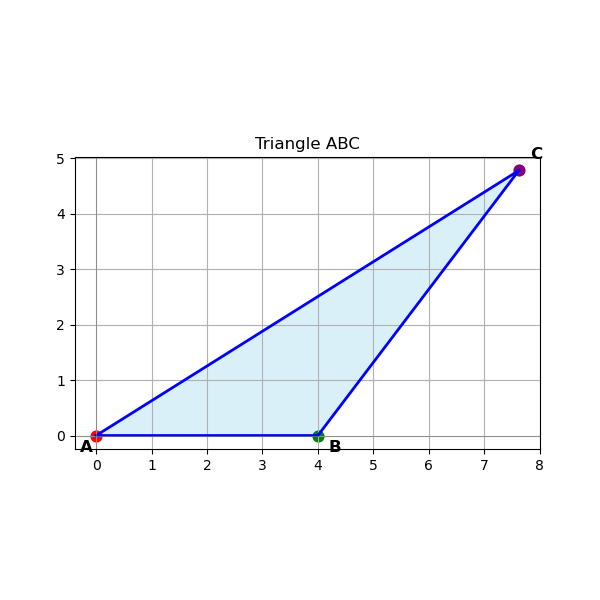
\includegraphics[width=\columnwidth, height=0.8\textheight, keepaspectratio]{Figure_5.png}     
\end{frame}
\end{document}